\section{Solution Issues for Reaction Term}

% % Copyright (C) 2007 Technical University of Liberec.  All rights reserved.
%
% Please make a following refer to Flow123d on your project site if you use the program for any purpose,
% especially for academic research:
% Flow123d, Research Centre: Advanced Remedial Technologies, Technical University of Liberec, Czech Republic
%
% This program is free software; you can redistribute it and/or modify it under the terms
% of the GNU General Public License version 3 as published by the Free Software Foundation.
%
% This program is distributed in the hope that it will be useful, but WITHOUT ANY WARRANTY;
% without even the implied warranty of MERCHANTABILITY or FITNESS FOR A PARTICULAR PURPOSE.
% See the GNU General Public License for more details.
%
% You should have received a copy of the GNU General Public License along with this program; if not,
% write to the Free Software Foundation, Inc., 59 Temple Place - Suite 330, Boston, MA 021110-1307, USA.

\normalsize

%%%%%%%%%%%%%%%%%        DOCUMENTATION OF GENERAL KINETIC REACTION FOR FUTURE -START           %%%%%%%%%%%%%%%

% \subsection{General Kinetic Reaction}
% \label{sec:kinetic}
% We consider a system of $m$ stoichiometric reactions, each symbolically written as
% \begin{equation} \label{eqn:general_kinetic_reaction}
%   \sum\limits_{i=1}^{n_r} \nu_{rik}\chi_{i} \rightarrow \sum\limits_{i=1}^{n_r} \nu_{pik} \chi_{i},
% \end{equation}
% where 
% \begin{itemize}
%   \item $\nu_{rik}$ \units{}{}{} is the stoichiometric coefficient (number of moles) 
%         for reactant component $i$ in reaction $k$,
%   \item $\nu_{pik}$ \units{}{}{} is the stoichiometric coefficient
%         for product component $i$ in reaction $k$,
%   \item $n_r$ is the number of reaction components (both reactants and products),
%   \item $\chi_{i}$ represents the chemical symbol for the component $i$.
% \end{itemize}
% For the components that are not present in reaction, the stoichiometric coefficients are set
% $\nu_{rik}=0$ or $\nu_{pik}=0$.
% 
% The kinetics temperature dependence is introduce in modified Arrhenius model.
% The production rate of the component $i$ is then modeled as
% \begin{equation} \label{eqn:modified_arrhenius}
%   \frac{\d c_i}{\d t} = M_i \sum\limits_{k=1}^{m}\left( \nu_{pik}-\nu_{rik} \right) 
%   B_k \left(\frac{T}{T_{0k}}\right)^{\alpha_k} \exp\left(-\frac{\Delta E_k}{R_gT}\right)
%   \prod\limits_{j=1}^{n_r}\left(\frac{\rho_j}{M_j}\right)^{\nu_{rjk}},
% \end{equation}
% where
% \begin{itemize}
%   \item $c_i$ \units{1}{-3}{} is concentration of component $i$,
%   \item $M_i$, $M_j$ \units{1}{-3}{} is the molar mass of component $i$, or $j$ respectively,
%   \item $B_k$ \units{}{}{-1} is the collision-frequency factor (or preexponential factor) of reaction $k$,
%               it represents number of all particle collisions per second (not all necessarilly 
%               resulting in reaction),
%   \item $T$ [K] is the current absolute temperature,
%   \item $T_{0k}$ [K] is the reference absolute temperature, at which the number of particle collisions per second
%         is equal $B_k$,
%   \item $\alpha_k$ \units{}{}{} is the temperature exponent of the reaction $k$,
%   \item $\Delta E_k$ $[\textrm{Jmol}^{-1}]$ is the activation energy per mole,
%   \item $R_g = 8.3144$ $[\textrm{Jmol}^{-1}\textrm{K}^{-1}]$ is the universal gas constant,
%   \item $\rho_j$ \units{1}{-3}{} is the density of component $j$.
% \end{itemize}
% 
% To get rid of the unit dependence on the exponent, we divide the equation \eqref{eqn:modified_arrhenius} 
% by liquid density $\rho=\sum_{j=1}^{n_r}\rho_i$ and put $M_i$ under the exponent. Using
% \begin{equation}
%   \prod\limits_{j=1}^{n_r}\left( \frac{\rho_j M_i}{\rho M_j}\right)^{\nu_{rjk}} 
%   = \left(\frac{M_i}{\rho}\right)^{\sum_{j=1}^{n_r}\nu_{rjk}} 
%     \prod\limits_{j=1}^{n_r}\left( \frac{\rho_j}{M_j}\right),
% \end{equation}
% we obtain
% \begin{equation}
%   \frac{\d}{\d t}\left(\frac{c_i}{\rho}\right) = \sum\limits_{k=1}^{m}\left( \nu_{pik}-\nu_{rik} \right) 
%   B_k \left(\frac{T}{T_{0k}}\right)^{\alpha_k} \exp\left(-\frac{\Delta E_k}{R_gT}\right)
%   \left(\frac{M_i}{\rho}\right)^{1-\sum_{j=1}^{n_r}\nu_{rjk}} 
%   \prod\limits_{j=1}^{n_r}\left( \frac{\rho_j M_i}{\rho M_j}\right)^{\nu_{rjk}} 
% %   
% %   = \left(\frac{M_i}{\rho}\right)^{\sum_{j=1}^{n_r}\nu_{rjk}} 
% %     \prod\limits_{j=1}^{n_r}\left( \frac{\rho_j}{M_j}\right),
% \end{equation}

%%%%%%%%%%%%%%%%%          DOCUMENTATION OF GENERAL KINETIC REACTION FOR FUTURE -END           %%%%%%%%%%%%%%%

\subsection{Radioactive Decay}
\label{sec:decay}
The radioactive decay is one of the processes that can be modelled in the reaction term of the transport model.
This process is coupled with the transport using the operator splitting method.
It can run throughout all the phases, including the mobile and immobile phase of the liquid 
and also the sorbed solid phase, as it can be seen in figure \ref{fig:reaction_term}.

The radioactive decay of a parent radionuclide A to a nuclid B
%
\[ A\xrightarrow{k} B, \qquad A\xrightarrow{t_{1/2}} B \]
%
is mathematicaly formulated as a system of first order differential equations
%
\begin{eqnarray} \label{eqn:halflife}
  \frac{\d c_A}{\d\tau} &=& -k c_A, \\
  \frac{\d c_B}{\d\tau} &=& k c_A,
\end{eqnarray}
%
where $k$ is the radioactive decay rate. Usually, the half life of the parent radionuclide \hyperA{Decay::half-life}{$t_{1/2}$} 
is known instead of the rate. Relation of these can be derived:
%
% \begin{equation} \label{eqn:halflife}
%   k = - \frac{\ln 2}{t_{1/2}}.
% \end{equation}
\begin{eqnarray*}
    \frac{\d c_A}{\d\tau} &=& -k c_A\\
    \frac{\d c_A}{c_A} &=& -k \d\tau\\
    \int\limits_{c_A^0}^{c_A^0/2}\frac{\d c_A}{c_A} &=& -k\int\limits_{0}^{t_{1/2}} 1\d\tau\\
    \big[ \ln c_A\big]^{c_A^0/2}_{c_A^0} &=& -\big[k\tau\big]^{t_{1/2}}_{0}\\
    \ln\frac{c_A^0}{2} - \ln c_A^0 &=& - k t_{1/2}\\
    \ln 2 &=& k t_{1/2}\\
    k &=& \frac{\ln 2}{t_{1/2}}.
\end{eqnarray*}

Let us now suppose a more complex situation. Consider substances (radionuclides) $A_1,\ldots, A_s$ which take 
part in a complex radioactive chain, including branches, e.g.
\begin{center}
\begin{tabular}{rccll}
 $A_1\xrightarrow{k_1}A_2\xrightarrow{k_2}$ & $A_3$ & $ \xrightarrow{k_{34}}$ & $A_4\xrightarrow{k_4}$ & $A_8$ \\
 & $A_3$ & $\xrightarrow{k_{35}} A_5 \xrightarrow{k_{5}}$ & $A_4$ &\\
 & $A_3$ & \multicolumn{2}{c}{$\xrightarrow{k_{36}} A_6 \xrightarrow{k_{6}} A_7 \xrightarrow{k_{7}}$} & $A_8$
\end{tabular}
\end{center}
Now the problem turned into a system of differential equations $\partial_t \vc{c}=\mathbf{D}\vc{c}$ with the following
matrix, generally full and nonsymmetric:
\[
\mathbf{D} = \begin{pmatrix} -k_1 &k_{21}& \cdots & k_{s1} \\ 
                  k_{12} & -k_2 & \cdots & k_{s2} \\
                  \vdots &\vdots& \ddots & \vdots \\
                  k_{1s} &k_{2s}& \cdots & -k_s \end{pmatrix}
\]
We denote the rate constant of an $i$-th substance 
\[
  k_i=\sum_{j=1}^{s}k_{ij}=\sum_{j=1}^{s}b_{ij}k_i
\]
which is equal to a sum of partial rate constants $k_{ij}$. Branching ratio \hyperA{RadioactiveDecayProduct::branching-ratio}{$b_{ij}$}$\in(0,1)$ 
determines the distribution into different branches of the decay chain, holding $\sum_{j=1}^{s}b_{ij}=1$.

Notice, that physically it is not possible to create a chain loop, so in fact one can permutate the vector of 
concentrations and rearrange the matrix $D$ into a lower triangle matrix
\[
\mathbf{D} = \begin{pmatrix} -k_1 &  &  &  \\ 
                  k_{12} & -k_2 & &  \\
                  \vdots &\vdots& \ddots &  \\
                  k_{1s} &k_{2s}& \cdots & -k_s \end{pmatrix}.
\]
However, we do not do this and we do not search the reactions for chain loops.

The system of first order differential equations with constant coefficients is solved using one of the
implemented ODE solvers.


\subsection{First Order Reaction}
\label{sec:first_order_reaction}
First order kinetic reaction is another process that can take part in the reaction term. Similarly to the
radioactive decay, it is connected to transport by operator splitting method and can run in all the possible
phases, see figure \ref{fig:reaction_term}.

Currently, reactions with single reactant and multiple products (decays) are available in the software.
The mathematical description is the same as for the radioactive decay, it only uses kinetic reaction rate
coefficient \hyperA{Reaction::reaction-rate}{$k$} in the input instead of half life.







% OLD
% The software suppports linear chemical reactions in the transport operator splitting method. 
% The linear chemical reactions (we will recall them only as 'reactions' in this section) can desribe
% \begin{itemize}
%   \item first order kinetic chemical reactions
%   \item radioactive decays, their chains and also complex chains with branches.
% \end{itemize}
% In the first case, the kinetics of a reaction is determined by a kinetic constant \hyperA{Substep::kinetic}{$k$}. 
% In the second case, the radioactive decay is determined by the half life of the reactant 
% \hyperA{Substep::half-life}{$t_{1/2}$}. Both notations
% %
% \[ A\xrightarrow{k} B, \qquad A\xrightarrow{t_{1/2}} B \]
% %
% express the same reaction and are governed by the same first order differential equation 
% %
% \[ \frac{\d c_A}{\d\tau} = -kc_A = - \frac{\ln 2}{t_{1/2}}\, c_A. \]
% %
% The relation between $k$ and $t_{1/2}$ is derived below
% \begin{eqnarray*}
%     \frac{\d c_A}{\d\tau} &=& -k c_A\\
%     \frac{\d c_A}{c_A} &=& -k \d\tau\\
%     \int\limits_{c_A^0}^{c_A^0/2}\frac{\d c_A}{c_A} &=& -k\int\limits_{0}^{t_{1/2}} 1\d\tau\\
%     \big[ \ln c_A\big]^{c_A^0/2}_{c_A^0} &=& -\big[k\tau\big]^{t_{1/2}}_{0}\\
%     \ln\frac{c_A^0}{2} - \ln c_A^0 &=& - k t_{1/2}\\
%     \ln 2 &=& k t_{1/2}\\
%     k &=& \frac{\ln 2}{t_{1/2}}.
% \end{eqnarray*}
% 
% 
% 
% Lets consider to have a narrow decay chain without branches. This kind of decay chain can be described by following equation
% \[
%  A\xrightarrow{t_{1/2,A}}B\xrightarrow{t_{1/2,B}}C\xrightarrow{t_{1/2,C}}D\xrightarrow{t_{1/2,D}}E,
% \]
% where letters $\{A,\ldots, E\}$ denotes isotopes contained in considered decay chain and ${t_{1/2},i},~i\in\{A,\ldots, E\}$ is a symbol for a half-life of $i$-th isotope.
% For a simulation of radioactive decay and first order reactions matrix multiplication based approach has been developed. It has been based on an arrangement of all the data to matrices. The matrix ${\bf C}^k$ contains the information about concentrations of all species ($s$) in all observed elements ($e$). The upper index $k$ denotes $k$-th time step. The matrix ${\bf C}^k$ has the dimension $e\times s~( rows \times columns)$.
% The transport simulation is realized by matrix multiplication 
% \[
%   {\bf T}\cdot{\bf C}^k = {\bf C}^{k+1},
% \]
% where ${\bf T}$ is a square, block-diagonal matrix, representing a set of algebraic equations constructed from a set of partial differential equations.
% When the simulation of the radioactive decay or the first order reaction is switched on, one step of
% simulation changes to 
% \[
%   {\bf T}\cdot{\bf C}^k\cdot{\bf R} = {\bf C}^{k+1},
% \]
% where ${\bf R}$ is a square matrix with the dimension $(s \times s)$ . It is much easier to construct and to use ${\bf R}$ , than to include chemical influence to the transport
% matrix ${\bf T}$ , because the matrix ${\bf R}$ has usually a simple structure and $s$ is much smaller than $e$. In the most simple case, when the order of identification numbers of isotopes in considered decay chain is the same as the order of identifiers of species transported by groundwater, then just two
% diagonals are engaged and the matrix R looks as follows:
% 
% \begin{tiny}\[
%    \begin{array}{l}
%     {\bf R} = \left(
%     \begin{array}{cccccc}
%      \left(\frac{1}{2}\right)^\frac{\Delta t}{t_{1/2,1}} & 1 - \left(\frac{1}{2}\right)^\frac{\Delta t}{t_{1/2,i}} & 0 & \hdots & \hdots & 0\\
%      0 & \left(\frac{1}{2}\right)^\frac{\Delta t}{t_{1/2,2}} & 1 - \left(\frac{1}{2}\right)^\frac{\Delta t}{t_{1/2,2}} & 0 & \ddots & 0 \\
%      \vdots & \ddots & \ddots & \ddots & \ddots & \vdots\\
%      0 & \ddots & 0 & \left(\frac{1}{2}\right)^\frac{\Delta t}{t_{1/2,n-2}} & 1 - \left(\frac{1}{2}\right)^\frac{\Delta t}{t_{1/2,n-2}} & 0 \\
%      0 & \hdots & \hdots & 0 & \left(\frac{1}{2}\right)^\frac{\Delta t}{t_{1/2,n-1}} & 1 - \left(\frac{1}{2}\right)^\frac{\Delta t}{t_{1/2,n-1}}\\
%      0 & \hdots & \hdots & 0 & 0 & 1
%     \end{array}\right)
%    \end{array}
% \]\end{tiny}
% 
% Every single $j$-th column, except the first one, includes the contribution $1 - \left(\frac{1}{2}\right)^\frac{\Delta t}{t_{1/2,j}},~j\in\{A,\ldots, E\}$ from $(j-1)$-th
% isotope with its half-life $t_{1/2,j-1}$. The term $\left(\frac{1}{2}\right)^\frac{\Delta t}{t_{1/2,j}}$ describes concentration decrease caused by the radioactive decay of $j$-th isotope itself. In general cases the matrix ${\bf R}$ can have much more complicated structure, especially when the considered decay chain has more branches.
% The implementation of the radioactive decay in Flow123D does not firmly include standard natural decay chain. Instead of that it is possible for a user to define his/her decay chain.
% 
% It is also possible to simulate decay chains with branches as picture \ref{pic:dec_branches} shows.
% 
% \begin{figure}[htb]
%  \centering
%  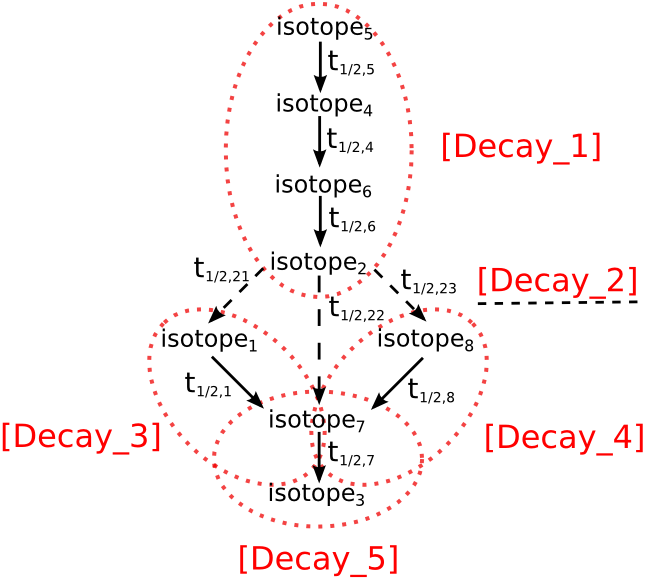
\includegraphics[width = 8cm]{\fig /decay_chain.png}
%  \caption{Decay chain with branches.}
%  \label{pic:dec_branches}
% \end{figure}
% 
% 
% When it comes to a simulation of first order reactions, the kinetic constant is given as an input. 
% The description of a kinetic chemical reaction has obviously two folowing forms
% \[
%   \begin{array}{l}
%     A\xrightarrow{k}B,\\
%     \frac{dc^A}{dt} = -k \cdot c^A.
%   \end{array}
% \]
% The first one description is a standard chemical one. The second equation describes temporal decrease in amount of concentrations of the specie $c^A$. The constant $k$ is so called kinetic constant and for the case of a first order reactions it is equal to so called reaction rate. The order of reaction with just one reactant is equal to the power of $c^A$ in partial diferential reaction.
% 
% For an inclusion of first order reaction into a reaction matrix a half-life needs to be computed from the corresponding kinetic constant $k$. The derivation follows
% \[
%   \begin{array}{l}
%     A\xrightarrow{k} B\\
%     \frac{dc^A}{d\tau} = -k\cdot c_A\\
%     \frac{dc^A}{c^A} = -k\cdot d\tau\\
%     \int\limits_{c^A_0/2}^{c^A_0}\frac{dc^A}{c^A} = -k\cdot\int\limits_{t_{1/2,A}}^{0} d\tau\\
%     \left[ ln c^A\right]_{c^A_0/2}^{c^A_0} = -[k\tau]_{t_{1/2,A}}^{0}\\
%     ln c^A_0 - \ln\frac{c^A_0}{2} = k\cdot t_{1/2,A}\\
% %     c^A (t) = c^A_0\cdot e^{-k\cdot t_{1/2,A}}\\
% %     {\bf substitution} \qquad c^A(t_{1/2,A}) = \frac{1}{2}\cdot c^A_0\\
% %     \frac{1}{2} c^A_0 = c^A_0\cdot e^{-k_1\cdot t_{1/2,A}}\\
%     \ln 2 = k \cdot t_{1/2,A}\\
%     t_{1/2,A} = \frac{ln 2}{k}
%   \end{array}                                                                                                                                                                                                                                                                                                            
% \]
% The matrix ${\bf R}$ is constructed in the same way as for the radioactive
% decay.


\subsection{Dual Porosity} 
\label{sec:num_dual_porosity}

The analytic solution of the system of differential equations \eqref{eq:odes_dual_por} at the time $t$ with initial conditions $c_m(0)$ and $c_i(0)$ is
\begin{align}
     c_m(t) &= (c_m(0) - c_a(0)) \exp\left(- D_{dp}\left(\frac{1}{\vartheta_m} + \frac{1}{\vartheta_i}\right) t \right) + c_a(0), 
     \label{eqn:dual_porosity_anal1}\\
     c_i(t) &= (c_i(0) - c_a(0)) \exp\left(- D_{dp}\left(\frac{1}{\vartheta_m} + \frac{1}{\vartheta_i}\right) t \right) + c_a(0),
     \label{eqn:dual_porosity_anal2}
\end{align}
where $c_a$ is the weighted average
\[
  c_a = \frac{\vartheta_m c_m + \vartheta_i c_i}{\vartheta_m + \vartheta_i}.
\]

If the time step is large, we use the analytic solution to compute new values of concentrations. 
Otherwise, we replace the time derivatives in \eqref{eqn:dual_porosity_ode1} and \eqref{eqn:dual_porosity_ode2} 
by first order forward differences and we get the classical Euler scheme
\begin{subequations}
\label{eq:dp_expl_euler}
\begin{align}
  c_m(t^+) = \frac{D_{dp} \Delta t}{\vartheta_m}(c_i(t) - c_m(t)) + c_m(t), \\
  c_i(t^+) = \frac{D_{dp} \Delta t}{\vartheta_i}(c_m(t) - c_i(t)) + c_i(t), \\
\end{align}
\end{subequations}
where $\Delta t = t^+ - t$ is the time step. 

The condition on the size of the time step is derived from the Taylor expansion of 
\eqref{eqn:dual_porosity_anal1} or \eqref{eqn:dual_porosity_anal2}, respectively. We neglect the higher order 
terms and we want the second order term to be smaller than the given \hyperA{DualPorosity::scheme-tolerance}{scheme tolerance} 
$tol$, relatively to $c_a$,
\begin{equation}
  (c_m(0) - c_a(0))
  \frac{ D_{dp}^2 (\Delta t)^2 \left(\frac{\vartheta_m + \vartheta_i}{\vartheta_m \vartheta_i}\right)^2}{2}
  \frac{1}{c_a} \leq tol. \\
\end{equation}
We then transform the above inequation into the following condition which is tested in the program
\begin{equation} \label{eqn:euler_scheme_condition}
  \max(|c_m(0) - c_a(0)|, |c_i(0) - c_a(0)|) \leq 
  2 c_a \left(\frac{\vartheta_m \vartheta_i}{D_{dp} \Delta t (\vartheta_m + \vartheta_i)}\right)^2 tol. \\
\end{equation}
In addition, the explicit Euler method \eqref{eq:dp_expl_euler} requires the satisfaction of a CFL condition of the form
\begin{equation}
\label{eq:dp_cfl}
\Delta t \le \frac1{D_{dp}} \frac{\th_m \th_i}{\th_m+\th_i}.
\end{equation}
If either of the inequalities \eqref{eqn:euler_scheme_condition} or \eqref{eq:dp_cfl} is not satisfied, then the analytic 
solution is used.


\subsection{Equilibrial Sorption}
\label{sec:num_sorp_math}

Let us now describe the actual computation of the sorption model.
To solve \eqref{eq:nonlin_sorption} iteratively, it is very important to define the interval where 
to look for the solution (unknown $c_l$), see Figure \ref{fig:sorpce}. The lower bound is $0$ (concentration can not reach negative values). 
The upper bound is derived using a simple mapping. Let us suppose limited 
\hyperA{Sorption::solubility}{solubility} of the selected transported substance and let us denote the 
limit $\bar{c}_l$. We keep the maximal "total mass" 
$\bar{c}_T= \mu_l\cdot \bar{c}_l + \mu_s\cdot f(\bar{c}_l)$, but we dissolve all the mass to get 
maximal $c_l^{max} > \bar{c}_l$. That means $c_s = 0$ at this moment. We can slightly enlarge the interval by setting the upper bound equal to 
$c_l^{max} + const_{small}$.

\begin{figure}[ht!]
 \centering
 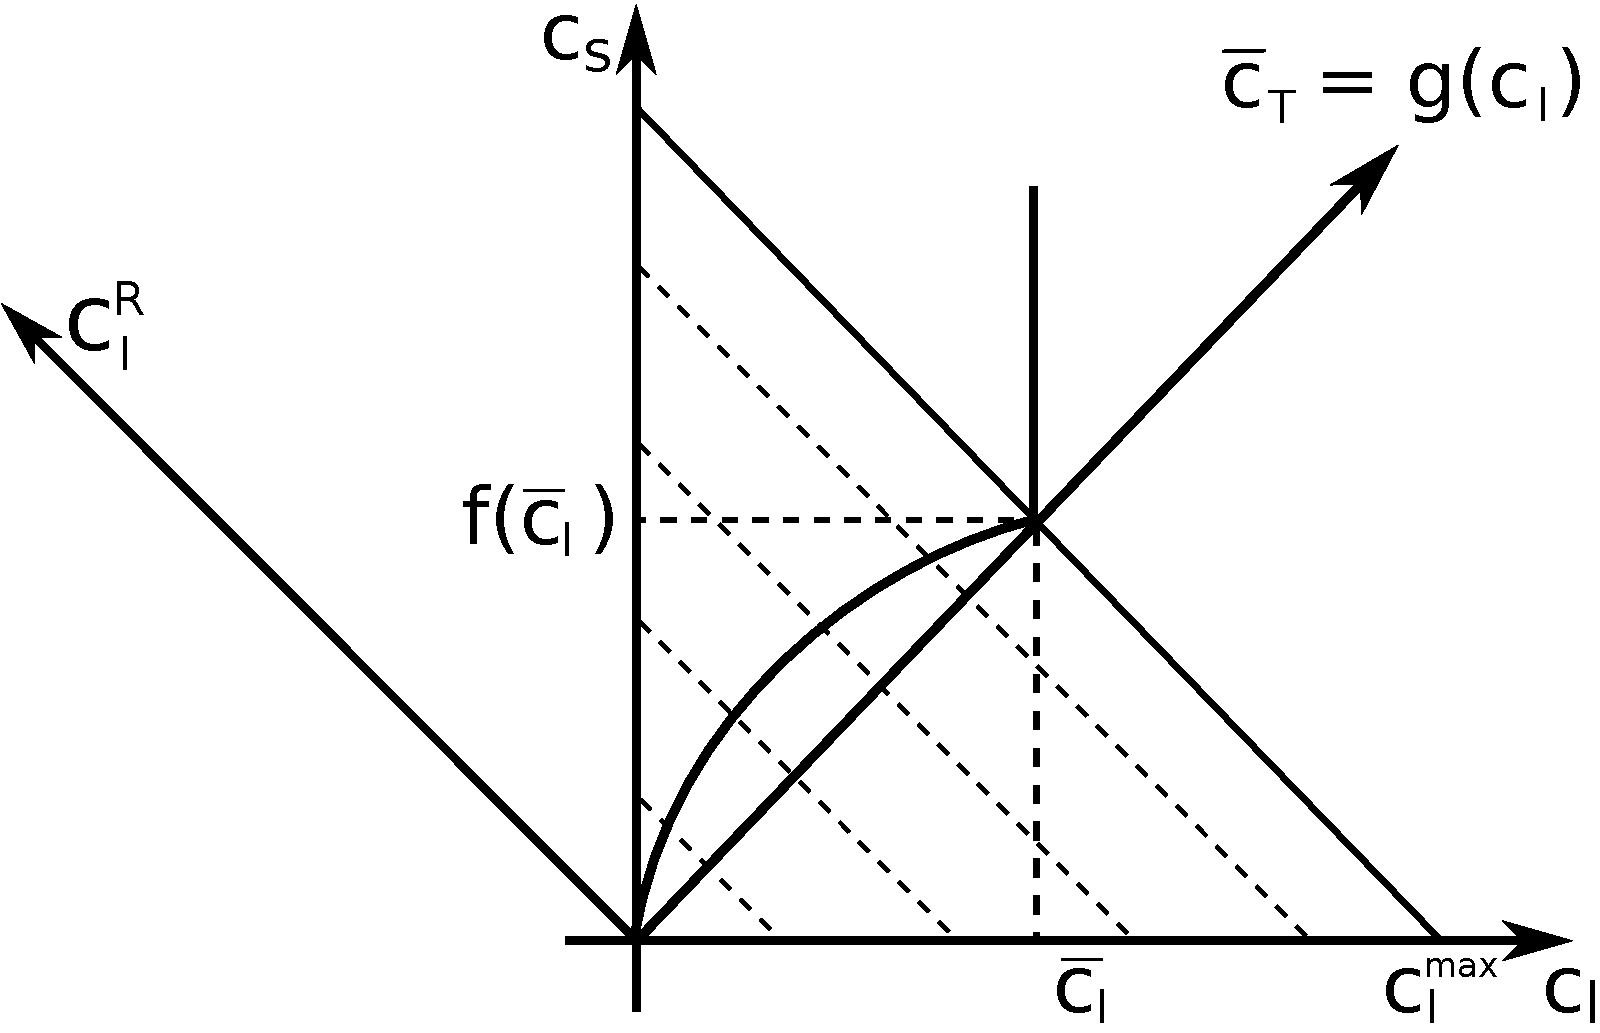
\includegraphics[width = 0.75\textwidth]{\fig/sorpce.pdf}
 \caption{Sorption in combination with limited solubility.}
 \label{fig:sorpce}
\end{figure}


To approximate the equation \eqref{eq:nonlin_sorption} using interpolation, we need to prepare the set of values 
which represents $[c_l, f(c_l)]$, with $c_l$ equidistantly distributed in transformed (rotated and rescaled) 
coordination system at first. The construction process of the interpolation table follows.
\begin{enumerate}
 \item Maximal ``total mass'' $\bar{c}_T = \mu_l\cdot \bar{c}_l + \mu_s\cdot f(\bar{c}_l)$ is computed.
 \item Total mass step is derived $mass\_step = \bar{c}_T/n\_steps$. $n\_steps$ is the number of
       \hyperA{Sorption::substeps}{substeps}.
 \item Appropriate $c_T^j = (mass\_step\cdot j)/\mu_l,~j\in \{0,\ldots, n\_steps\}$ are computed. 
 \item The equations $\mu_l \cdot c_T^j = \mu_l\cdot c_l^j + \mu_s\cdot f(c_l^j)~j\in \{0,\ldots, n\_steps\}$ are solved 
       for $c_l^j$ as unknowns. The solution is the set of ordered couples (points) 
       $[c_l^j,f(c_l^j)],~j\in\{0,\ldots,n\_steps\}$.
\end{enumerate}
After the computation of $\{[c_l^j,f(c_l^j)]\}$, we transform these coordinates to the system where the total mass is 
an independent variable. This is done by multiplication of precomputed points using the transformation matrix ${\bf A}$:
\begin{equation}
 \begin{array}{l}
  \vec{c}\,^R = {\bf A}\cdot\vec{c}\\
  \left[\begin{array}{c} c_l^{R,j}\\ c_s^{R,j} \end{array}\right] = 
  \left[\begin{array}{cc}
    \vartheta\cdot \rho_w & M_s(1 - \vartheta)\rho_R\\
    -M_s(1 - \vartheta)\rho_R & \vartheta\cdot \rho_w
  \end{array}\right]\cdot
  \left[\begin{array}{c} c_l^j\\ c_s^j \end{array}\right]\\
  j\in\{0,\ldots,n\_steps\}
 \end{array}
 \label{eq:transf_mat}
\end{equation}

The values $c_l^{R,j}$ are equidistantly distributed and there is no reason to save them, but the values 
$c_s^{R,j}$ are stored in onedimensional interpolation table.

Once we have the interpolation table, we can use it for projecting the transport results ${[c_l,c_s]}$ on the 
isotherm under consideration. Following steps must be taken.
\begin{enumerate}
 \item Achieved concentrations are transformed to the coordinate system through multiplication with the 
       matrix ${\bf A}$, see \eqref{eq:transf_mat}.
 \item Transformed values are interpolated.
 \item The result of interpolation is transformed back. The backward transformation consists of multiplication 
       with ${\bf A}^T$ which is followed by rescaling the result. Rescaling the result is necessary because  
       ${\bf A}$ is not orthonormal as it is shown bellow.
 \[
 \begin{array}{l}
 {\bf A}^T\cdot{\bf A} =
  \left((\vartheta - 1)^2\cdot M_s^2\cdot \rho_R^2 + \vartheta^2\cdot \rho_w^2\right)\cdot\left[\begin{array}{cc}
    1 & 0\\
    0 & 1
  \end{array}\right]
  \end{array}
 \]
\end{enumerate}


% \subsection{Limited Solubility}\label{subsec:lim_solub}
\paragraph{Limited solubility.} When $\mu_l\cdot c_l + \mu_s\cdot f(c_l) > \mu_l\cdot \bar{c}_l + \mu_s\cdot f(\bar{c}_l)$, neither iterative 
solver nor interpolation table is used. The aqueous concentration is set to be $\bar{c}_l$ and sorbed 
concentration is computed $c_s = (\mu_l\cdot c_l + \mu_s\cdot f(c_l) - \mu_l\cdot \bar{c}_l)/\mu_s$.

\subsection{System of Linear Ordinary Differential Equations}
\label{sec:num_slode}

A system of linear ordinary differential equations (ODE) appears in several places in the model. 
Let us denote the ODE system
\[
  \partial_t \vc c(t) = \mathbf{A}(t) \vc{c}(t) + \vc{b}(t).
\]

For the moment the only implemented method to solve the system is usage of Pad\'e approximant which corresponds to a family
of implicit R-K methods.

% \paragraph{Semi-analytic solution.}
% A semi-analytic solution can be obtained in special cases due to the physical nature of the problem.
% The problem can be then solved only by a~matrix multiplication $\vc c(t+\Delta t) = \mathbf{R} \vc{c}(t)$. 
% This is used in case of radioactive decays and first order kinetic reactions.
% 
% The right hand side $\vc{b}$ is zero and $\mathbf{A}$ is constant. The assumption is made that the equations 
% are independent during one time step. Each quantity $c_i$ (concentration in this case) is decreased 
% by $e^{a_{ii} \Delta t}$ (supposing negative diagonal) during time step $\Delta t$. The decrement $\left( 1-e^{a_{ii} \Delta t} \right)$
% is then distributed among other quantities according to the given fraction.
% 
% In case of radioactive decays and first order reactions, the elements of the solution matrix $\mathbf{R}$ are
% \begin{eqnarray*}
%      r_{ii} &=& e^{-k_i \Delta t}, \\
%      r_{ji} &=& \left( 1-e^{-k_i \Delta t} \right) b_{ji} \frac{M_j}{M_i},
% \end{eqnarray*}
% where $b_{ji}$ is the branching ratio of $i$-th reactant (or radionuclide) and $\frac{M_j}{M_i}$ is 
% the fraction of molar masses.
% The expressions $b_{ji} \frac{M_j}{M_i}$ are then obtained from the system matrix by dividing 
% $-\frac{a_{ji}}{a_{ii}}$. See the system matrix entries in \eqref{eqn:reaction_system_entries}.
% 
% The assumption (equations independence) is adequate when a very small time step is applied. This will then lead 
% to huge amount of evaluations of the exponential functions which can be expensive, so other numerical methods 
% might be more appropriate. When the time step is large then the assumption is inadequate.
% 
% On the other hand, if the time step is constant (for significantly large number of time steps), we get the
% solution cheaply just by matrix multiplication, because the matrix $\mathbf{R}$ is constant.


\paragraph{Pad{\' e} approximant.}
For homogenous systems with constant matrix $\mathbf{A}$, we can use \hyperA{IT::PadeApproximant}{Pad{\' e} approximation} 
to find the solution. This method finds a rational function whose power series agrees with a power series expansion of 
a given function to the highest possible order (e.g. in \cite{press_numerical_1992}).
Let
\[
  f(t) = \sum\limits_{j=0}^{\infty} c_j t^j = \sum\limits_{j=0}^{\infty} \frac{1}{n!}f^{(j)}(t_0)
\]
be the function being approximated and its power series given by Taylor expansion about $t_0$.
Then the rational function
\begin{equation} \label{eqn:pade_approximant}
R_{mn}(t) = \frac{P_m(t)}{Q_n(t)} = \frac{\sum\limits_{j=0}^{m} p_jt^j}{\sum\limits_{j=0}^{n} q_jt^j},
\end{equation}
which satisfies 
\begin{equation} \label{eqn:pade_coef_equations}
f(t)\approx \sum\limits_{j=0}^{m+n} c_j t^j = R_{mn}(t),
\end{equation}
% \begin{equation} \label{eqn:pade_coef_equations}
% \sum\limits_{j=0}^{m+n} c_jt^j \sum\limits_{j=0}^{m} q_jt^j = \sum\limits_{j=0}^{n} p_jt^j,
% \end{equation}
is called Pad{\' e} approximant. From \eqref{eqn:pade_coef_equations}, we obtain $m+n+2$ equations for
coefficients of the nominator $P_m$ (polynomial of \hyperA{PadeApproximant::pade-nominator-degree}{degree} $m$) and 
the denominator $Q_n$ (polynomial of \hyperA{PadeApproximant::pade-denominator-degree}{degree} $n$). We also see that the error 
of the approximation is $O(t^{m+n+1})$. By convention, the denominator is normalized such that $q_0=1$.
Theoretical results show that for $m=n-1$ and $m=n-2$ the Pad\'e approximant corresponds to an implicit Runge-Kutta method
which is A-stable and L-stable (see \cite{ehle1973}).

Now, we consider the solution of our ODE system in a form $\vc{c}(t)=e^{\mathbf{A}t}\vc{c}(0)$. We shall 
approximate the matrix exponential function using a matrix form of \eqref{eqn:pade_approximant}. 
For exponential functions, there are known coeffficients of the nominator and denominator:
% http://mathoverflow.net/questions/41226/pade-approximant-to-exponential-function
% http://www.math.vanderbilt.edu/~esaff/texts/144.pdf
% https://www-sop.inria.fr/apics/anap03/PadeTalk.pdf
\begin{eqnarray}
  \mathbf{P}_m(\mathbf{A}t) &=& \sum\limits^{m}_{j=0}\frac{(m+n-j)!m!}{(m+n)!j!(m-j)!} (\mathbf{A}t)^j, \\
  \mathbf{Q}_n(\mathbf{A}t) &=& \sum\limits^{n}_{j=0} (-1)^j \frac{(m+n-j)!n!}{(m+n)!j!(n-j)!} (\mathbf{A}t)^j.
\end{eqnarray}
Finally, we can write the solution at time $t+\Delta t$
\begin{equation} \label{eqn:pade_solution}
\vc{c}(t+\Delta t) = \frac{\mathbf{P}_m(\mathbf{A}\Delta t)} {\mathbf{Q}_n(\mathbf{A}\Delta t)}\vc{c}(t) 
= \mathbf{R}_{mn}(\mathbf{A}\Delta t)\vc{c}(t).
\end{equation}

If the time step $\Delta t$ is constant, we do not need to compute the matrix $\mathbf{R}_{mn}$ repeatedly and we get
the solution cheaply just by matrix multiplication. In the oposite case, we avoid evaluating the exponential
function and still get the solution quite fast (comparing to computing semi-analytic solution).